% !TEX program = xelatex
\documentclass[UTF8,a4paper,zihao=5,fontset=none]{ctexart}

\usepackage[a4paper,margin=22mm,headheight=15pt,footskip=12mm]{geometry}
\usepackage{amsmath}
\usepackage{array}
\usepackage{booktabs}
\usepackage{caption}
\usepackage{enumitem}
\usepackage{fancyhdr}
\usepackage{float}
\usepackage{graphicx}
\usepackage{hyperref}
\usepackage{listings}
\usepackage{longtable}
\usepackage{microtype}
\usepackage{tabularx}
\usepackage[table]{xcolor}

\IfFileExists{/System/Library/Fonts/Supplemental/Arial Unicode.ttf}{
  \setCJKmainfont[Path=/System/Library/Fonts/Supplemental/,AutoFakeBold=2]{Arial Unicode.ttf}
  \setCJKsansfont[Path=/System/Library/Fonts/Supplemental/,AutoFakeBold=2]{Arial Unicode.ttf}
  \setCJKmonofont[Path=/System/Library/Fonts/Supplemental/]{Arial Unicode.ttf}
}{
  \setCJKmainfont{FandolSong-Regular}
  \setCJKsansfont{FandolHei-Regular}
  \setCJKmonofont{FandolFang-Regular}
}

\definecolor{accent}{HTML}{176B87}
\definecolor{deepblue}{HTML}{17324D}
\definecolor{lightrow}{HTML}{F3F7F8}
\definecolor{codebg}{HTML}{F4F6F7}
\definecolor{rulegray}{HTML}{A8B6C2}

\hypersetup{
  colorlinks=true,
  linkcolor=accent,
  urlcolor=accent,
  pdfauthor={敖炜},
  pdftitle={Gemma 3 270M 的 SVG 徽标 LoRA 微调实验},
  pdfsubject={LoRA 训练、奖励函数与基座对比分析}
}

\pagestyle{fancy}
\fancyhf{}
\fancyfoot[L]{\color{gray}\small Gemma 3 270M SVG 徽标 LoRA 实验}
\fancyfoot[R]{\color{gray}\small\thepage}
\renewcommand{\headrulewidth}{0pt}
\renewcommand{\footrulewidth}{0pt}

\ctexset{
  section={format=\Large\bfseries\color{accent},beforeskip=1.1em,afterskip=0.55em},
  subsection={format=\large\bfseries\color{deepblue},beforeskip=0.8em,afterskip=0.4em}
}
\setlength{\parindent}{2em}
\setlength{\parskip}{0.25em}
\setlength{\emergencystretch}{2em}
\setlist[itemize]{leftmargin=2em,itemsep=0.15em,topsep=0.3em}
\renewcommand{\arraystretch}{1.18}
\captionsetup{font=small,labelfont=bf}

\newcolumntype{Y}{>{\centering\arraybackslash}X}
\newcommand{\thead}[1]{\cellcolor{accent}\color{white}\bfseries #1}
\newcommand{\repo}{https://github.com/ao-wei/gemma3-270m-svg-lora-partb}
\newcommand{\caseimage}[1]{\includegraphics[width=0.96\linewidth,height=31mm,keepaspectratio]{#1}}

\lstdefinestyle{reportcode}{
  basicstyle=\ttfamily\scriptsize,
  backgroundcolor=\color{codebg},
  frame=single,
  rulecolor=\color{rulegray},
  breaklines=true,
  columns=fullflexible,
  keepspaces=true,
  showstringspaces=false,
  xleftmargin=0.5em,
  xrightmargin=0.5em,
  aboveskip=0.5em,
  belowskip=0.5em
}

\begin{document}

\thispagestyle{fancy}
\vspace*{27mm}
\begin{center}
  {\fontsize{24}{34}\selectfont\bfseries\color{deepblue}
    Gemma 3 270M 的 SVG 徽标\\[2mm]LoRA 微调实验\par}
  \vspace{19mm}
  \renewcommand{\arraystretch}{1.45}
  \begin{tabularx}{0.82\textwidth}{>{\bfseries}p{28mm}X}
    \rowcolor{accent}\color{white}姓名 & \color{white}敖炜 \\
    学号 & 202521080810 \\
    \rowcolor{lightrow}日期 & 2026-07-14 \\
    GitHub & {\small\url{\repo}} \\
  \end{tabularx}
\end{center}
\vfill
\clearpage

\section*{摘要}

我在 Apple M4 上使用 Transformers 和 PEFT 对 Gemma 3 270M 进行 LoRA 微调。原始训练集有 219 条记录，其中两条只含冲突的 placeholder，因此仅在加载时过滤，不改动源文件。17 条验证数据一直保留到最后，没有用于选择学习率、epoch、随机种子或 checkpoint。前期的三图元模型作为预热；最终模型从该权重出发，用全部 217 条完整 SVG 继续训练一轮。

主模型将 fatal rate 从 100.0\% 降到 0.0\%，总 reward 从 0.0235 提高到 0.3638。但 fidelity 只从 0.0509 变为 0.0621，配对置信区间跨过 0；quality pass rate 也仍为 0.0\%。结合全部渲染图，我把结论限定为“SVG 格式稳定性有提升，提示保真和视觉质量没有得到可靠改善”。

\section{数据边界与训练方法}

训练加载器使用模型自带 chat template；system、user 与 padding token 的标签全部为 -100，仅 assistant SVG token 参与交叉熵。完整 chat 最大长度为 3535，最终 \texttt{max\_length=3584}，所有最终训练记录零截断。LoRA rank=4、alpha=16、dropout=0.05，仅作用于 \texttt{q\_proj/k\_proj/v\_proj/o\_proj}；batch size=1、梯度累积=8、梯度检查点开启。训练是监督微调，reward 只用于内部选择和分析，并非 RL。

为了在 16GB MPS 上保留完整 SVG，训练使用精确的分块词表投影损失：按 token 块计算 lm\_head 与交叉熵，再按有效 assistant token 总数归一化。数值检查与原始全 logits loss 的绝对差为 0。\\\texttt{precision:auto} 仅对明确 BF16 算子不兼容错误重启 FP32；OOM 不会伪装成兼容问题。

\section{Reward v3 与 pass 定义}

总分公式为 $0.30\times$语法安全 $+ 0.20\times$几何 $+ 0.15\times$结构样式 $+ 0.25\times$提示保真 $+ 0.10\times$反退化。提示保真内部为颜色 45\%、图形 25\%、空间 20\%、构图 10\%；不存在可靠空间要求时对其他分项重新归一化。空间关系只在元素可唯一匹配时评分，歧义标记 unscorable。stroke-width 必须有限、非负且不超过 viewBox 短边 10\%。

权重的考虑如下：
\begin{itemize}
  \item 语法与安全占 30\%，因为无法解析或含脚本的 SVG 根本不能作为徽标使用，应首先失去大部分分数。
  \item 几何占 20\%，用来区分“XML 可解析”和“画布上真有内容”；负坐标、非有限数和异常粗的线条都会使可见结果失效。
  \item 结构与样式占 15\%，奖励可见图元和合理调色，但不让难以程序化判断的“美观”主导总分。
  \item 提示保真占 25\%，它直接对应作业目标，但颜色和图形关键词只是语义的近似，因此权重低于语法与几何之和。
  \item 反退化占 10\%，专门阻止截断、重复片段和模板泄漏等容易“刷分”的行为。
\end{itemize}

\begin{itemize}
  \item valid pass：非 fatal 且 validity $\geq 0.8$。
  \item quality pass：valid pass、total $\geq 0.5$、fidelity $\geq 0.3$，且无背景/空白退化。
  \item 致命 XML/安全错误有总分上限；背景、画布外与重复退化进入 violations。
\end{itemize}

\section{E0--E14 实验过程}

\small
\begin{longtable}{>{\centering\arraybackslash}p{8mm}p{27mm}>{\centering\arraybackslash}p{6mm}>{\centering\arraybackslash}p{14mm}>{\centering\arraybackslash}p{15mm}>{\centering\arraybackslash}p{10mm}>{\centering\arraybackslash}p{10mm}>{\centering\arraybackslash}p{15mm}>{\centering\arraybackslash}p{12mm}}
\toprule
\thead{实验} & \thead{变量/目标} & \thead{r} & \thead{训练/开发} & \thead{lr} & \thead{长度} & \thead{epoch} & \thead{eval loss} & \thead{秒} \\
\midrule
\endfirsthead
\toprule
\thead{实验} & \thead{变量/目标} & \thead{r} & \thead{训练/开发} & \thead{lr} & \thead{长度} & \thead{epoch} & \thead{eval loss} & \thead{秒} \\
\midrule
\endhead
E0 & default r=8 & 8 & 110/22 & 2.0e-04 & 2048 & 1.0 & 1.1858 & 513.7 \\
\rowcolor{lightrow}E1 & rank 4 & 4 & 110/22 & 2.0e-04 & 2048 & 1.0 & 1.1824 & 524.3 \\
E2 & rank 16 & 16 & 110/22 & 2.0e-04 & 2048 & 1.0 & 1.1859 & 559.7 \\
\rowcolor{lightrow}E3 & lr=1e-4 & 8 & 110/22 & 1.0e-04 & 2048 & 1.0 & 1.3055 & 562.4 \\
E4 & lr=5e-4 & 8 & 110/22 & 5.0e-04 & 2048 & 1.0 & 1.0509 & 551.9 \\
\rowcolor{lightrow}E5 & length 3072 & 8 & 110/22 & 2.0e-04 & 3072 & 1.0 & 1.3901 & 632.1 \\
E6 & 195 rows, 4 epochs & 4 & 195/22 & 5.0e-04 & 2048 & 4.0 & 0.7251 & - \\
\rowcolor{lightrow}E7 & seed 123 & 4 & 195/22 & 5.0e-04 & 2048 & 1.0 & 0.9051 & - \\
E8 & shortest 110 & 4 & 110/22 & 2.0e-04 & 1536 & 3.0 & 0.9573 & 670.9 \\
\rowcolor{lightrow}E9 & 6 elements & 4 & 195/22 & 2.0e-04 & 1536 & 3.0 & 0.7196 & 705.4 \\
E10 & 3 elements & 4 & 195/22 & 2.0e-04 & 1024 & 2.0 & 0.6773 & 356.7 \\
\rowcolor{lightrow}E11 & full SVG, lr=5e-5 & 4 & 195/22 & 5.0e-05 & 3584 & 1 & 1.0408 & 826.1 \\
E12 & full SVG, lr=1e-4 & 4 & 195/22 & 1.0e-04 & 3584 & 1 & 0.9875 & 659.7 \\
\rowcolor{lightrow}E13 & full SVG, seed 42 & 4 & 217/0 & 5.0e-05 & 3584 & 1 & - & 788.7 \\
E14 & full SVG, seed 123 & 4 & 217/0 & 5.0e-05 & 3584 & 1 & - & 661.4 \\
\bottomrule
\end{longtable}
\normalsize

E0--E5 分别比较了 rank、学习率和长度上限。rank 4 与 rank 8/16 的开发 loss 差别很小，因此后续使用参数更少的 rank 4。E4 在早期筛选中 loss 最低，但后续生成检查显示，仅靠 loss 不能保证 SVG 完整。

E6--E10 尝试了更多样本、更多 epoch、按长度排序以及六图元/三图元派生目标。E6/E7 的摘要是从 checkpoint 重载后记录的，不把其十余秒耗时当作完整训练时间。E10 的三图元模型成为最终完整 SVG 训练的初始权重，但不是最终提交模型。

E11/E12 只在固定 22 条内部开发集比较。E12 的 fatal rate 为 31.8\%，且 fidelity 没有改善，因此按事先设定的门槛选择 E11 的 lr=5.0e-05。E13/E14 都从 E10 权重出发，用全部 217 条完整 SVG 训练；seed 42 是主结果，seed 123 只用于检查稳健性。

\begin{table}[H]
\centering
\small
\begin{tabular}{lccc}
\toprule
\thead{最终阶段} & \thead{峰值 MPS driver memory} & \thead{最大序列} & \thead{截断} \\
\midrule
E11 & 3.85 GiB & 3535 / 3584 & 0 \\
\rowcolor{lightrow}E12 & 3.85 GiB & 3535 / 3584 & 0 \\
E13 & 3.84 GiB & 3535 / 3584 & 0 \\
\rowcolor{lightrow}E14 & 3.82 GiB & 3535 / 3584 & 0 \\
\bottomrule
\end{tabular}
\end{table}

\section{最终 17 条验证结果}

\begin{table}[H]
\centering
\small
\begin{tabular}{lrrrrrr}
\toprule
\thead{模型} & \thead{total} & \thead{validity} & \thead{fidelity} & \thead{fatal rate} & \thead{valid pass} & \thead{quality pass} \\
\midrule
Base & 0.0235 & 0.0688 & 0.0509 & 100.0\% & 0.0\% & 0.0\% \\
\rowcolor{lightrow}Stage1（三图元） & 0.2882 & 0.7028 & 0.1890 & 17.6\% & 64.7\% & 0.0\% \\
E13 seed42 & 0.3638 & 0.7539 & 0.0621 & 0.0\% & 11.8\% & 0.0\% \\
\rowcolor{lightrow}E14 seed123 & 0.3432 & 0.7045 & 0.0383 & 5.9\% & 5.9\% & 0.0\% \\
\bottomrule
\end{tabular}
\end{table}

seed42 相对 base 的配对结果：

\begin{table}[H]
\centering
\small
\begin{tabular}{lccc}
\toprule
\thead{指标} & \thead{均值差} & \thead{bootstrap 95\% CI} & \thead{改善/持平/退化} \\
\midrule
total & 0.3402 & [0.3088, 0.3795] & 17/0/0 \\
\rowcolor{lightrow}validity & 0.6852 & [0.6146, 0.7475] & 17/0/0 \\
fidelity & 0.0113 & [-0.0631, 0.0864] & 7/7/3 \\
\bottomrule
\end{tabular}
\end{table}

\section{典型样本与 Goodhart}

我逐条检查了 17 组 reference/base/seed42/seed123 图像。seed42 视觉有效 0/17、背景单图元 2/17；seed123 视觉有效 0/17、背景单图元 1/17。下面四例分别展示格式改善但视觉仍空白、单背景退化、代理分高估和随机种子不稳定。

\subsection{样本 0}
\begin{table}[H]
\centering
\begin{tabularx}{\textwidth}{YYYY}
\caseimage{output/cases/sample_00_reference.png} & \caseimage{output/cases/sample_00_base.png} & \caseimage{output/cases/sample_00_seed42.png} & \caseimage{output/cases/sample_00_seed123.png} \\
参考 & 基座 & seed 42 & seed 123
\end{tabularx}
\end{table}
base / seed42 / seed123 的 total 为 0.1000 / 0.3500 / 0.3500；fidelity 为 0.2733 / 0.1042 / 0.1042。微调前的输出无法作为单一 SVG 解析；两个最终模型虽然生成了完整 XML，但图元集中在负坐标并反复复制。语法改善是真实的，画面仍为空白。

\subsection{样本 4}
\begin{table}[H]
\centering
\begin{tabularx}{\textwidth}{YYYY}
\caseimage{output/cases/sample_04_reference.png} & \caseimage{output/cases/sample_04_base.png} & \caseimage{output/cases/sample_04_seed42.png} & \caseimage{output/cases/sample_04_seed123.png} \\
参考 & 基座 & seed 42 & seed 123
\end{tabularx}
\end{table}
base / seed42 / seed123 的 total 为 0.0000 / 0.3500 / 0.3500；fidelity 为 0.0000 / 0.1042 / 0.1042。两个最终模型都只留下一个铺满画布的圆，主体水果和叶片消失。该例说明颜色或标签命中不能代替完整构图。

\subsection{样本 6}
\begin{table}[H]
\centering
\begin{tabularx}{\textwidth}{YYYY}
\caseimage{output/cases/sample_06_reference.png} & \caseimage{output/cases/sample_06_base.png} & \caseimage{output/cases/sample_06_seed42.png} & \caseimage{output/cases/sample_06_seed123.png} \\
参考 & 基座 & seed 42 & seed 123
\end{tabularx}
\end{table}
base / seed42 / seed123 的 total 为 0.0000 / 0.5837 / 0.5837；fidelity 为 0.0000 / 0.1250 / 0.1250。seed 42 的程序化总分是 0.5837，为验证集中最高值之一，但实际渲染为空白。无效 polygon 属性和画布外坐标造成了最明显的代理指标高估。

\subsection{样本 7}
\begin{table}[H]
\centering
\begin{tabularx}{\textwidth}{YYYY}
\caseimage{output/cases/sample_07_reference.png} & \caseimage{output/cases/sample_07_base.png} & \caseimage{output/cases/sample_07_seed42.png} & \caseimage{output/cases/sample_07_seed123.png} \\
参考 & 基座 & seed 42 & seed 123
\end{tabularx}
\end{table}
base / seed42 / seed123 的 total 为 0.0000 / 0.3500 / 0.0000；fidelity 为 0.0000 / 0.4062 / 0.0000。seed 42 生成了橙色圆盘，保真度代理分达到 0.4062，但提示中的深色徽章与中央火焰人物均未出现；seed 123 同一条样本又发生 XML 解析错误，显示训练结果对随机种子敏感。

\clearpage
\section{全部 17 条视觉审计}

\begin{figure}[H]
\centering
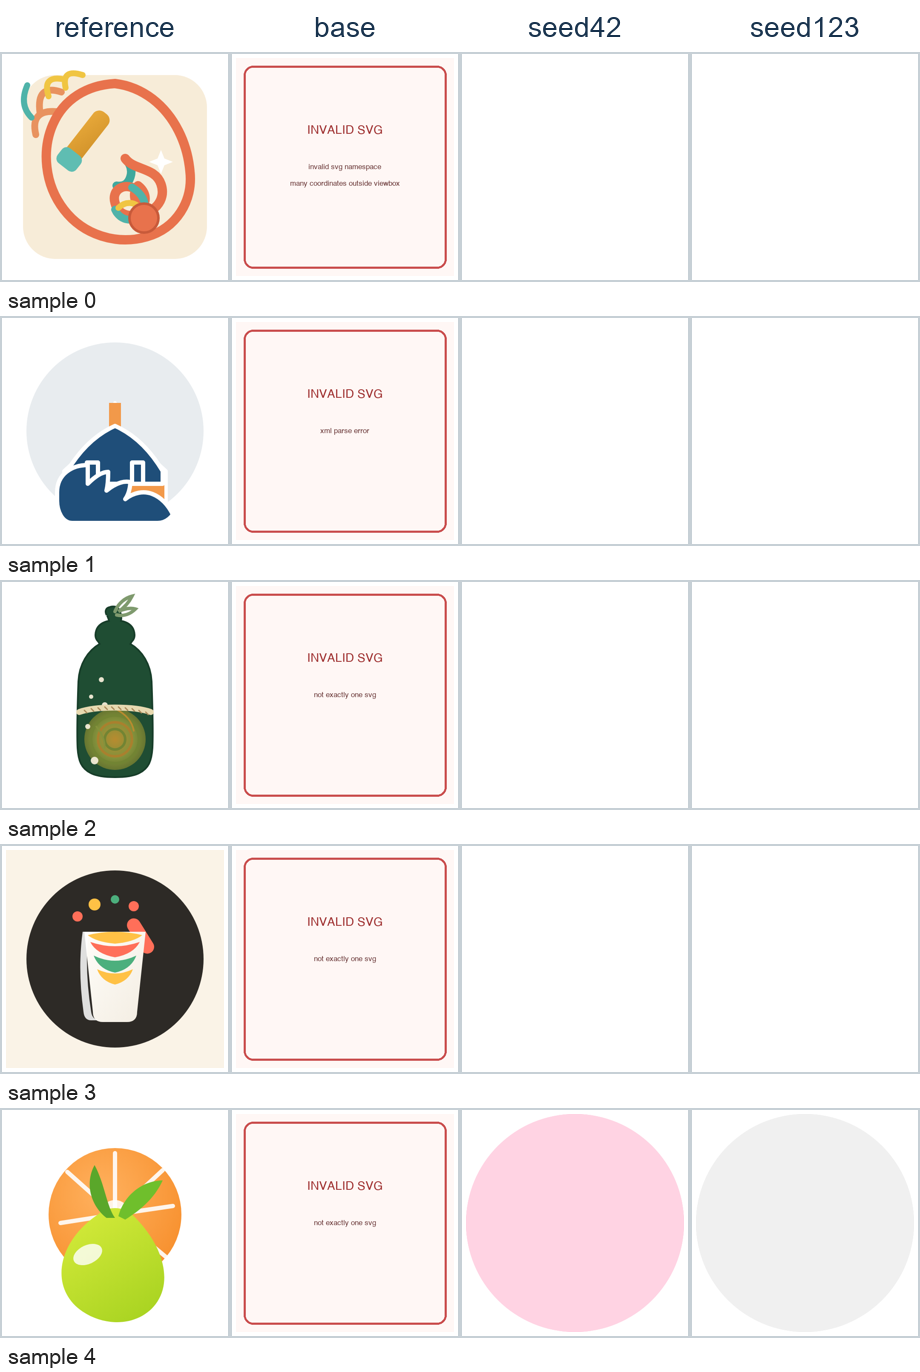
\includegraphics[width=\textwidth,height=0.85\textheight,keepaspectratio]{output/audit/contact_sheet_1.png}
\end{figure}
\clearpage

\begin{figure}[H]
\centering
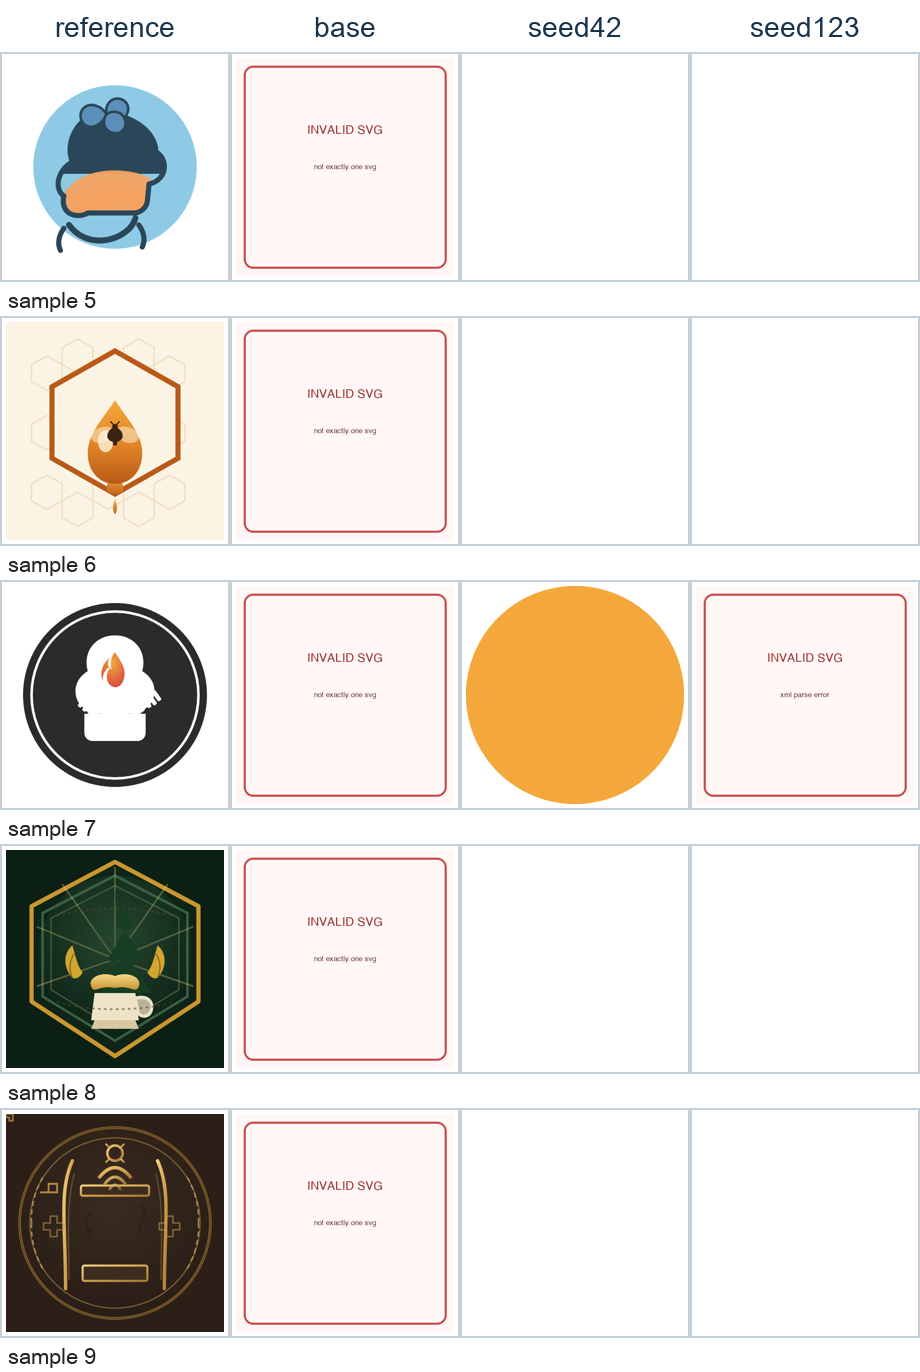
\includegraphics[width=\textwidth,height=0.88\textheight,keepaspectratio]{output/audit/contact_sheet_2.png}
\end{figure}
\clearpage

\begin{figure}[H]
\centering
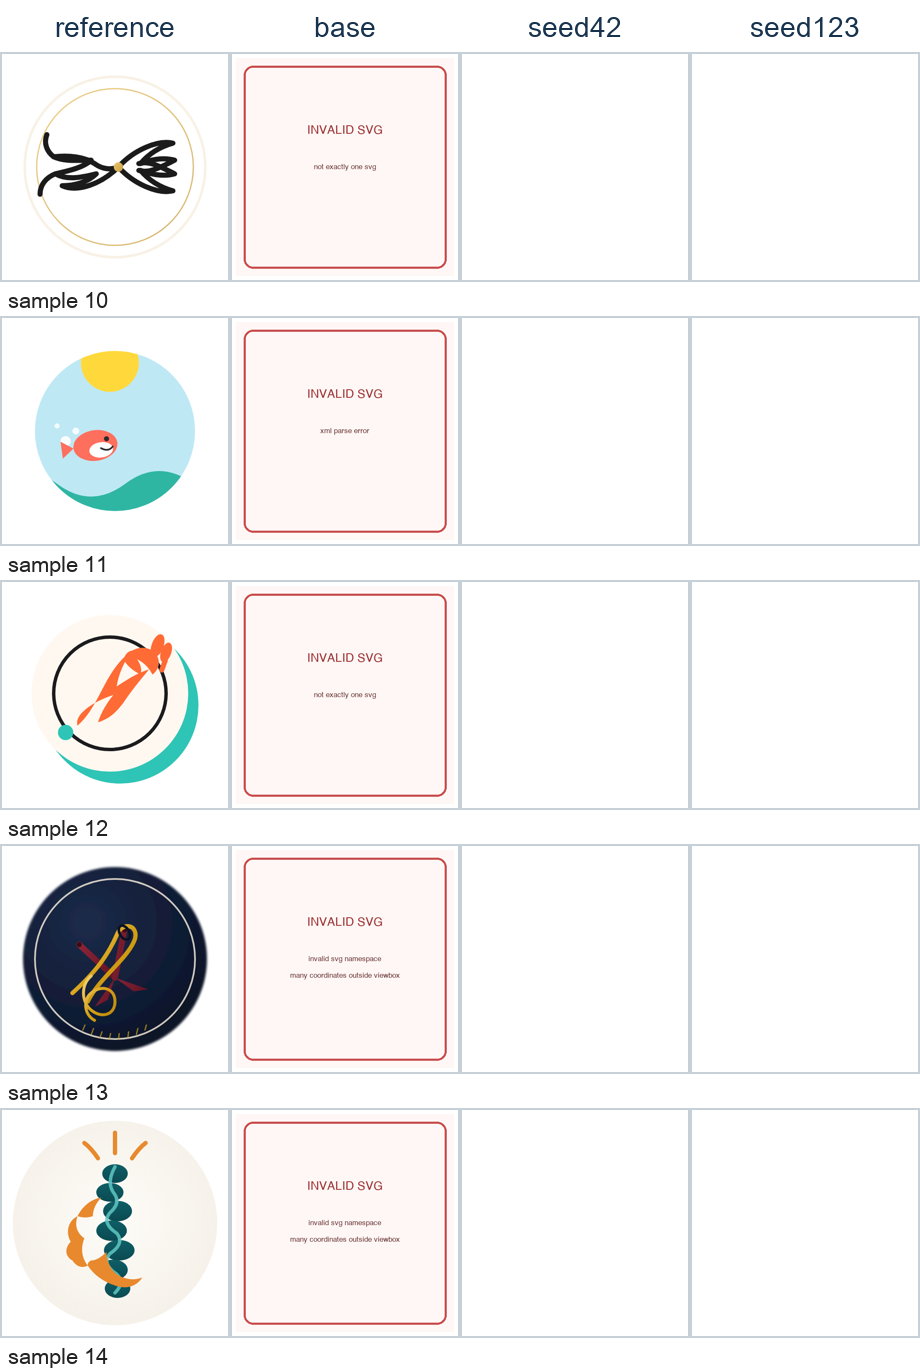
\includegraphics[width=\textwidth,height=0.88\textheight,keepaspectratio]{output/audit/contact_sheet_3.png}
\end{figure}
\clearpage

\begin{figure}[H]
\centering
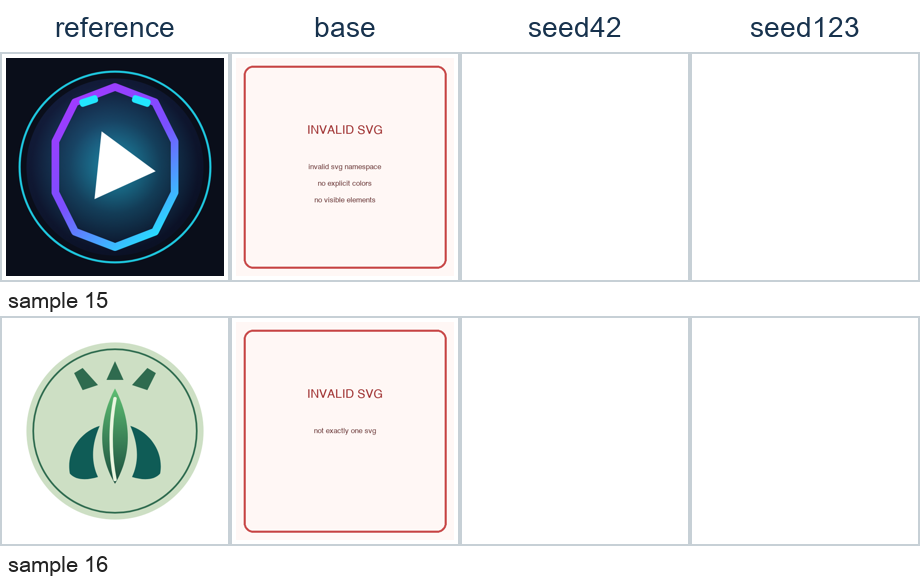
\includegraphics[width=\textwidth,height=0.75\textheight,keepaspectratio]{output/audit/contact_sheet_4.png}
\end{figure}

\section{结论与局限}

完整 SVG 继续训练确实把 seed42 的 fatal rate 降至 0，并且 34 个独立复验输出全部一致；但模型学习到的是高度重复、坐标为负的模板，几乎没有前景落在画布内。fidelity 的配对置信区间跨 0，两个 seed 的 quality pass 都为 0。270M 容量、长 SVG token 序列与纯文本交叉熵共同限制了语义构图。后续应采用更强基座、语法约束解码、结构化 SVG 表示和基于栅格图像的感知损失/评测。

\section{复现与验收}

\begin{lstlisting}[style=reportcode]
uv venv --python 3.12 .venv
uv pip install --python .venv/bin/python -r requirements.txt
.venv/bin/python -m unittest discover -s tests -v
.venv/bin/python student_kit/train_peft.py --config train_config.yaml
.venv/bin/python student_kit/eval_self.py --adapter adapter --output results.json
.venv/bin/python student_kit/analyze_results.py results.json
.venv/bin/python student_kit/build_visual_audit.py
.venv/bin/python student_kit/verify_artifacts.py --results results.json --repro runs/repro_full.json --adapter adapter
\end{lstlisting}

验收：测试 27/27；新进程 adapter 加载=True；schema v2=True；确定性复验 base 17/17、tuned 17/17。

GitHub 仓库：\url{\repo}

\clearpage
\appendix
\section{最终 train\_config.yaml}

\begin{lstlisting}[style=reportcode]
model_path: gemma3-270m-it
train_file: train.jsonl
output_dir: runs/e13_full217_seed42
init_adapter_path: adapter_curriculum_stage1
seed: 42
dev_size: 0
max_train_samples: null
drop_uninformative_prompts: true
simplify_targets: false
require_no_truncation: true
max_length: 3584
eval_max_length: 3584
precision: auto
auto_precision_fallback: true
batch_size: 1
gradient_accumulation_steps: 8
gradient_checkpointing: true
loss_chunk_size: 256
num_train_epochs: 1
learning_rate: 5.0e-05
weight_decay: 0.01
warmup_ratio: 0.05
lr_scheduler_type: cosine
max_grad_norm: 1.0
logging_steps: 5
eval_steps: 25
save_steps: 25
early_stopping: false
early_stopping_patience: 1
lora_r: 4
lora_alpha: 16
lora_dropout: 0.05
target_modules:
- q_proj
- k_proj
- v_proj
- o_proj
\end{lstlisting}

\section{哈希与结果 schema}

\begin{itemize}
  \item 主 adapter SHA-256：\par{\footnotesize\ttfamily 1ceedb3bfa3278a26e862b02b1933516a78c40586e8136c25dc78e9397cb64b5\par}
  \item train.jsonl SHA-256：\par{\footnotesize\ttfamily b8c90a46a0292bdfac3e0a9800f30bd8ceeacad05f0e3fab5a9de91ec84d8d18\par}
  \item valid.jsonl SHA-256：\par{\footnotesize\ttfamily 43f66b004843b91691d72c2949fb9dbf075408288d9a0a2a81a2337062bfce31\par}
  \item results schema v2：每条样本含 \path{raw_text}、\path{svg}、\path{reward}、\path{passes.valid}、\path{passes.quality}；汇总含 \path{pass_rate}、\path{valid_pass_rate}、\path{quality_pass_rate}。
  \item 关键产物：\path{results.json}、\path{results_seed123.json}、\path{results_stage1.json}、\path{render_manifest.json}、\path{manual_review.json}。
\end{itemize}

\end{document}
